% 本文中出现很多涉及到推理机制建模以及实验探究方法的专业名词,这里我们将对重点名词进行解释~\footnote{如果想了解更多key terms的定义,请参考\citet{InterpTermExplain_Blog}的工作。},如下表。
This paper introduces several specialized terms related to reasoning mechanism modeling and experimental exploration methods. Below, we provide explanations for the key terms \footnote{For more definitions of specialized terms, please refer to the work of \citet{InterpTermExplain_Blog}.}.

\begin{itemize}
    \item \textbf{Circuits}. Circuits are abstractions of the reasoning logic in deep models. The model $\mathcal{M}$ is viewed as a computational graph. There are two main approaches to modeling circuits. One approach treats the features in the latent space of $\mathcal{M}$ as nodes and the transitions between features as edges \citep{OldCircuit_20_distill_OpenAI}. The other approach views different components of $\mathcal{M}$, such as attention heads and neurons, as nodes; and the interactions between these components, such as residual connections, as edges \citep{IOI_23_ICLR_Redwood}. A circuit is a subgraph of $\mathcal{M}$. Current research on attention heads primarily uses the second definition.
    
    \item \textbf{Residual stream}. The residual stream after layer $\ell$ is the sum of the embedding and the outputs of all layers up to layer $\ell$, and is the input to layer $\ell+1$. \citet{MathFrame_21_TCT_Anthropic} offers a perspective of the residual stream as a shared bandwidth. Different layers can transmit information through this shared bandwidth (with lower layers writing information and higher layers reading it), as illustrated in Figure~\ref{fig:ResidualStream}.
    
    \item \textbf{Knowledge circuit}. As defined in \citep{KnowledgeCircuit_24_arXiv_ZJU}, a knowledge circuit is a critical subgraph in $\mathcal{M}$ to view the knowledge mechanism of Transformers. Knowledge circuits focus on how different components collaborate to express internal knowledge.
    
    \item \textbf{Activation patching} \& \textbf{Ablation study}. Activation patching involves replacing the activation values in certain layers of a model to analyze the contribution of these layers to the model's decision-making. Ablation study, on the other hand, involves removing a component from the LLM and observing the changes in the output \citep{ActivationPatching_24_arXiv_Google}.\\
    Both methods require calculating the effect towards output after the operation. Specifically, there are three types of effects: direct effect, indirect effect, and total effect, as shown in Figure~\ref{fig:ThreeEffect}.\\
    The key difference between them is that Activation Patching does not remove components, whereas Ablation Study logically removes a component.
    
    \item \textbf{Logit lens}. When calculating effects like those shown in Figure~\ref{fig:ThreeEffect}, logit lens can quantify this effect. Specifically, it uses uembedding layer to map an intermediate representation vector to the logits values of the vocabulary, allowing for the comparison of logits differences or other metrics~\citep{LogitLens_colab}.
\end{itemize}

\begin{figure}[htbp]
    \centering
    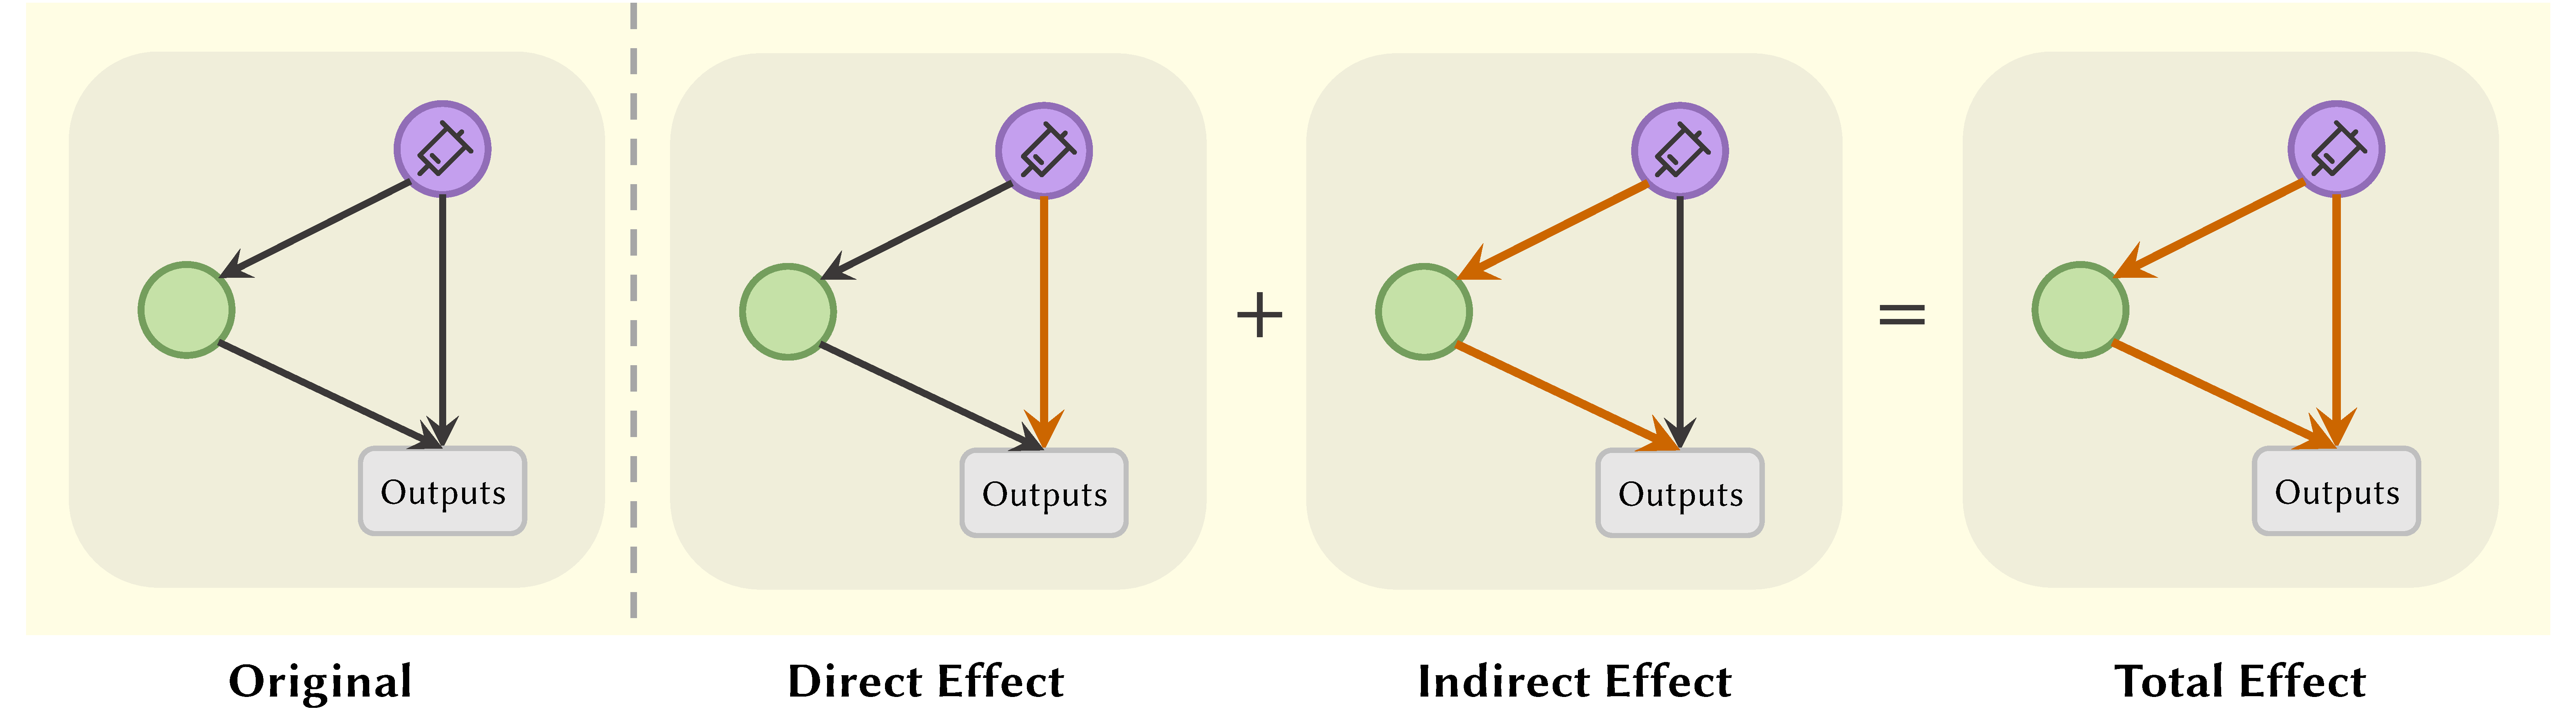
\includegraphics[width=0.9\linewidth]{figures/ThreeEffect.pdf}
    \caption{Three different types of calculating effects.}
    \label{fig:ThreeEffect}
\end{figure}